	\documentclass[11pt, a4paper]{article}
\usepackage[margin=2cm]{geometry}
\usepackage{helvet}
\usepackage{graphicx}
\usepackage{lineno}
\usepackage{breakcites}
\usepackage{hyperref}
\graphicspath{ { } }
\renewcommand{\familydefault}{\sfdefault}
\renewcommand{\baselinestretch}{1.5}




\begin{document}


Question 8:
 
\vspace{2cm} 
 
\includegraphics[scale=0.4]{question_8.pdf}
 
 
The systems coalesce towards monoculture / a lack of diversity as t approaches Inf, though it doesn't take too long to reach this state. This is because with each replacement in the system, there is an increasing chance that the larger species will replace another index in the community, under completely neutral / relaxed assumptions. The lack of diversification / new species as a secondary process to erode such monoculture also contributes to this.

\pagebreak

Question 12:

\vspace{2cm}


\includegraphics[scale=0.4]{question_12.pdf} 

Wherein a Maximal starting diversity is represented in red, and minimal is blue.


In this simulation, both a minimal and maximal diversity community quickly approach a shared discrete range of species richness values, and fluctuate to the same degree therein. This demonstrates the equilibrium of the system; lower richness promoting the generation of new species, and higher richness stifling these. With the same parametres both initial community vectors will end the same as the model simulates the same resources for each species regardless of starting vector, i.e. the same environment.

\newpage

Question 16

\includegraphics[scale=0.3]{question_16.pdf}

Wherein red represents maximal initial community diversity, blue minimal. X axis represents increasing octave index, binned up to x^2.

The initial state of the system herein does not seem to matter. There is very little difference between either barcharts / octave bins. Similarly, the biodiversity holding capacity of each simulation is the same, so either states fall to an easier to maintain equilibrium, even in terms of speciation.


\newpage

Question 21


For the “2D” square: There is a resizing factor of 3, and there are 8 exact replicates of the pattern here. Hence log(8)/log(3) =~ 1.8927

In “3D”, the resizing factor is constant; the entire tessaract is n+1 dimensions but so is the starting singular unit, hence  3. If there were to be taken 3*3*3 = 27 original “cubes” that may exist within the dimensional confines, there is clearly 1 cube missing from each side of this cube, plus an additional missing cube in the center in accordance with the scaling of the fractal pattern. Hence log(20)/log(3) =~ 2.726833 


Question 22

\includegraphics[scale=0.3]{chaos_game_21.pdf}

In this chaos game, the points do not simply plot either the entire plane between the 3 points randomly. Instead, a fractal is created spurred from the initial triangle.


\newpage

In the following graphs, these values were used: 
\vspace{1cm}

start_position <- c(0,0),  
direction <- pi/5,
length <- 3 

Question 25

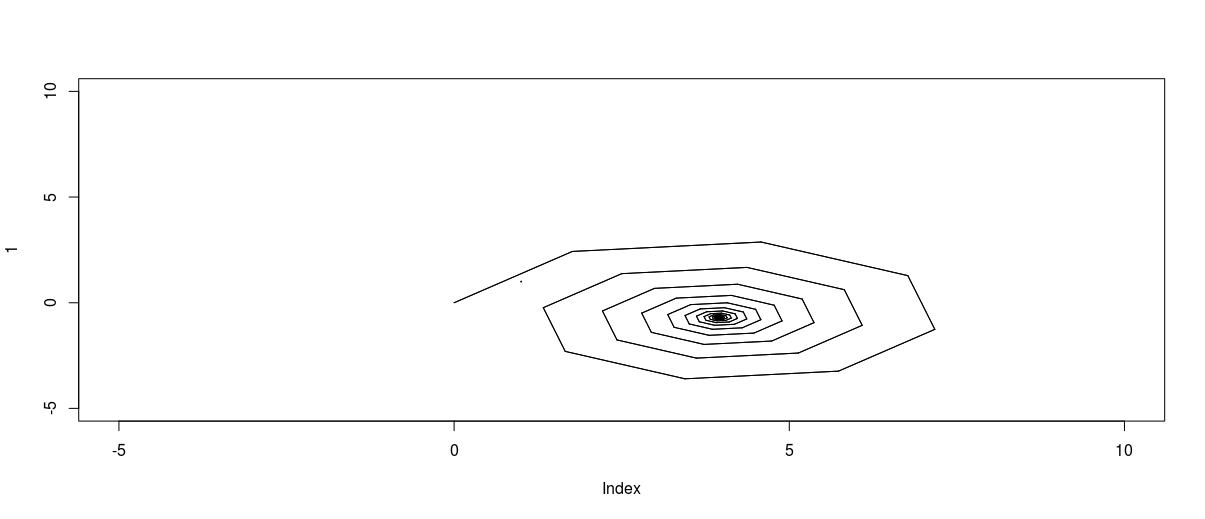
\includegraphics[scale=0.3]{spiral.pdf}

An error is given here:

\begin{verbatim}
Error: evaluation nested too deeply: infinite recursion / options(expressions=)?
\end{verbatim}
\vspace{1cm}

This is expected as the function is indeed infinitely calling upon itself, though the function manages to complete and "fill in" the center of the circle from our perspective before the r parser realises the infinite recursion.


Question 26

\includegraphics[scale=0.3]{spiral2.pdf}

By using "e" to limit line length, the infinite recursion is not a problem and no errors are created. Furthermore the	spiral can therefore be calibrated to stop at a given length, as in this example, where "e" is given to the function as 0.1.

\newpage

Question 27 
\includegraphics[scale=0.4]{tree.pdf} 

\end{document}